\newpage
\chapter{Neuronale Netze}
Tauchen Sie ein, in die wundersame Welt der k"unstlichen Intelligenz. \\
Ich beschreibe hier einen neuralen Netzwerk Simulator, der auch von nicht-technischen Leuten,
einfach zu verstehen ist.
Basierend auf backpropagation'es Lernen f"ur das hier vorgestellte Tool, ist es m"oglich,
Ihren Computer zu trainieren und zu lernen, was Sie von ihm erwarten. \\
Ich m"ochte Ihnen zugleich einen Vorrausblick geben, was uns in naher Zukunft erwartet. \\

\section{Arten von Netzwerken}
Folgende neurale Netzwerke, werde ich hier noch vorstellen:\\
* ein Netzwerk, um die Zahlen 1, 2, und 3 zu erkennen. \\
* ein Netzwerk, um die logische Funktion AND zu verarbeiten. \\
* ein Netzwerk, um die logische Funktion XOE zu verarbeiten. \\

\section{Was sind Neuronale Netzwerke ?}
Expert Definition: \\
Ein neurales Netzwerk ist eine parallel-laufende Informationsstruktur.

\chapter{Überwachtes Lernen}
Mit Lernen ist dabei die Fähigkeit gemeint, Gesetzmäßigkeiten nachzubilden.
Die Ergebnisse sind durch Naturgesetze oder Expertenwissen bekannt und werden benutzt,
um das System anzulernen.
\\
Ein Lernalgorithmus versucht, eine Hypothese zu finden, die möglichst zielsichere Voraussagen trifft. Unter Hypothese ist dabei eine Abbildung zu verstehen, die jedem Eingabewert den vermuteten Ausgabewert zuordnet. Dazu verändert der Algorithmus die freien Parameter der gewählten Hypothesenklasse. Oft wird als Hypothesenklasse die Menge aller Hypothesen, die durch ein bestimmtes künstliches neuronales Netzwerk modelliert werden kann, verwendet. In diesem Fall sind die frei wählbaren Parameter die Gewichte der Neuronen. Beim überwachten Lernen werden diese Gewichte derart angepasst, dass die Ausgabe der Neuronen denen eines vorgegebenen Teaching Vectors (engl., Lernvektor) möglichst nahekommt. Die Methode richtet sich also nach einer im Vorhinein festgelegten zu lernenden Ausgabe, deren Ergebnisse bekannt sind. Die Ergebnisse des Lernprozesses können mit den bekannten, richtigen Ergebnissen verglichen, also „überwacht“, werden. \\
\\
Um zu wissen, wann eine Hypothese zielsicher ist, wird ein Fehlermaß eingeführt, das minimiert werden soll. Eine beliebte Wahl ist der mittlere quadratische Fehler aller Trainingsdaten.

\section{Empirische Daten}
Empirie (vom griechischen: empeiría ‚Erfahrung, Erfahrungswissen) ist eine methodisch-systematische Sammlung von Daten. Auch die Erkenntnisse aus empirischen Daten werden manchmal kurz Empirie genannt.

\section{mittlerer quadratische Fehler}
Die mittlere quadratische Abweichung, auch der mittlere quadratische Fehler genannt und MQF oder MSE (aus dem englischen für mean squared error) abgekürzt, ist ein Begriff der mathematischen Statistik. Er gibt in der Schätztheorie an, wie sehr ein Punktschätzer um den zu schätzenden Wert streut. Damit ist er ein zentrales Qualitätskriterium für Schätzer.

\section{Punktschätzer}
Als Punktschätzer bezeichnet man eine Schätzfunktion, die jeder Stichprobe einen Wert zuordnet, der eine gewisse Eigenschaft des zugrundeliegenden Wahrscheinlichkeitsmaßes schätzen soll. In den meisten Anwendungen ist die interessierende Größe ein Parameter der Wahrscheinlichkeitsverteilung der Beobachtungen (wie z.B. der Mittelwert)

\section{Schätzfunktion}
Eine Schätzfunktion dient in der mathematischen Statistik dazu, aufgrund von vorhandenen empirischen Daten einer Stichprobe einen Schätzwert zu ermitteln und dadurch Informationen über unbekannte Parameter einer Grundgesamtheit zu erhalten. Schätzfunktionen sind die Basis zur Berechnung von Punktschätzungen und zur Bestimmung von Konfidenzintervallen mittels Bereichsschätzern und werden als Teststatistiken in Hypothesentests verwendet. Sie sind spezielle Stichprobenfunktionen und können durch Schätzverfahren, z. B. die Methode der kleinsten Quadrate  bestimmt werden.\\
Im Rahmen der Entscheidungstheorie können Schätzfunktionen auch als Entscheidungsfunktionen bei Entscheidungen unter Unsicherheit betrachtet werden.

\section{Grundgesamtheit}
Bezeichnet zum Beispiel die Gesamtheit von Populationen.
Die Menge aller Einheiten (auch Merkmalsträger, Untersuchungseinheit) mit übereinstimmenden Identifikationskriterien
(sachlich, räumlich und zeitgleich). \\
Die Einheit ist Träger der Informationen für die Untersuchung

\section{Stickprobe}
Als Stichprobe bezeichnet man eine Teilmenge einer Grundgesamtheit, die unter bestimmten Gesichtspunkten ausgewählt wurde.
\subsection{Auswahlverfahren}
Ein Auswahlverfahren ist die Art und Weise, wie die Elemente der Stichprobe möglichst zweckmäßig ausgewählt werden. Es gibt verschiedene Auswahlverfahren, die nachfolgend beschrieben werden.
\subsubsection{Zufallsauswahl}
Eine Zufallsstichprobe ist notwendig, wenn die Stichprobe repräsentativ sein soll, d. h. wenn von ihr nach dem Induktionsprinzip auf die Grundgesamtheit geschlossen werden soll, da es oft nicht möglich ist, die Grundgesamtheit (etwa die Gesamtbevölkerung oder alle Exemplare eines bestimmten Produkts) zu untersuchen.
\subsubsection{Bewusste Auswahl}
Bei einer systematischen Stichprobenziehung werden bereits bekannte Informationen über die auszuwählenden Fälle genutzt. Die Auswahl erfolgt anhand von Listen und festgelegten Regeln. Mathematisch-statistische Modelle, etwa die Berechnung der Einschlusswahrscheinlichkeit, sind bei bewussten Auswahlen nicht anwendbar. Systematische Auswahlverfahren kommen zum Beispiel im kommerziellen Bereich vor, wenn es auf Repräsentativität nicht ankommt.
\subsubsection{Willkürliche Auswahl}
Bei willkürlichen Stichproben werden Elemente aus der Grundgesamtheit (etwa von einem Interviewer) mehr oder weniger willkürlich in die Stichprobe aufgenommen. Die Auswahl liegt im Ermessen des Interviewers.

\section{Systematische Stischprobe}
Als Systematische Stichprobe (auch Bewusste Auswahl) bezeichnet man Auswahlverfahren, bei denen subjektive Erwägungen die Auswahl der Zielpersonen bestimmen.\\
\\
\textbf{Beispiel}: Alle Mitarbeiter mit mehr als 10 Jahren Betriebszugehörigkeit.\\
\\
Es werden Vorinformationen über die auszuwählenden Fälle genutzt. Verallgemeinerungen sind auf der Basis mathematisch-statistischer Modelle bei bewussten Auswahlen nicht möglich.

\section{Stichprobenvariable}
An dieser Stelle setzt die statistische Modellierung an. Die Stichprobenvariable ${\displaystyle X_{i}}$, eine Zufallsvariable, beschreibt mit ihrer Verteilung die Wahrscheinlichkeit, mit der eine bestimmte Merkmalsausprägung bei der i ${\displaystyle i}$ Ziehung aus der Grundgesamtheit auftritt. Jeder Beobachtungswert ${\displaystyle x_{i}}$ ist die Realisierung einer Stichprobenvariable ${\displaystyle X_{i}}$.

\section{Stichprobenfunktion}
Die Definition von Stichprobenvariablen ${\displaystyle X_{i}}$ erlaubt die Definition von Stichprobenfunktionen analog z. B. zu Kennwerten aus der deskriptiven Statistik:
\subsection{Arithmetisches Mittel - Formel}
{\Large{$\bar{\mathrm{x}} = \frac{x_1 + \ldots + x_n}{n}$}}
\subsection{Stichprobenfunktion - Formel}
{\Large{$\bar{\mathrm{X}} = \frac{X_1 + \ldots + X_n}{n}$}}

\section{Stichprobenverteilung}
Unter Stichprobenverteilung versteht man die Verteilung einer Stichprobenfunktion ${\displaystyle g(X_{1},\dotsc ,X_{n})}$ über alle möglichen Stichproben aus der Grundgesamtheit. Die Stichprobenfunktion ${\displaystyle g}$ ist in der Regel eine Schätzfunktion für einen unbekannten Parameter der Grundgesamtheit oder eine Teststatistik für eine Hypothese über einen unbekannten Parameter der Grundgesamtheit. Daher spricht man statt von Stichprobenverteilung auch einfach von der Verteilung einer Schätzfunktion oder Teststatistik. Die Verteilung der Stichprobenfunktion dient der Gewinnung von Aussagen über unbekannte Parameter in der Grundgesamtheit aufgrund einer Stichprobe.

\section{Hypothese}
In der Statistik bezeichnet man mit Hypothese eine Annahme, die mit Methoden der mathematischen Statistik auf Basis empirischer Daten geprüft wird. Man unterscheidet als Gegensatzpaar Nullhypothese und Alternativhypothese (auch Gegenhypothese). Häufig sagt die Nullhypothese aus, dass kein Effekt bzw. Unterschied vorliegt oder dass ein bestimmter Zusammenhang nicht besteht. Diese These soll verworfen werden, so dass die Alternativhypothese als Möglichkeit übrig bleibt. Durch dieses indirekte Vorgehen soll die Wahrscheinlichkeit für eine irrtümliche Verwerfung der Nullhypothese kontrolliert klein bleiben. Oft entsteht jedoch Verwirrung beim Anwender, weil dieses Vorgehen die Möglichkeit nahelegt, dass – sofern die Nullhypothese nicht verworfen und die Alternativhypothese damit nicht angenommen werden kann – die Nullhypothese als erwiesen gilt. Dies ist allerdings nicht der Fall.
\subsection{Alternativhypothese}
Als Alternativhypothese ${\displaystyle H_{1}}$ oder ${\displaystyle H_{A}}$ bezeichnet man in der empirischen Wissenschaft häufig eine durch Beobachtungen oder Überlegungen begründete Annahme oder Vermutung, die zur Erklärung bestimmter Phänomene dient und die einer möglicherweise verbreiteten Annahme oder Vermutung (nämlich der Nullhypothese) entgegensteht. Insofern kann die Alternativhypothese als innovativ betrachtet werden.\\
\\
Formal zerlegen die Null- und Alternativhypothese einen Parameterraum ${\displaystyle \Theta }$ in zwei disjunkte nicht leere Teilmengen ${\displaystyle \Theta _{0}}$ und ${\displaystyle \Theta _{1}}$. Die Nullhypothese beinhaltet die Aussage, dass der unbekannte Parameter ${\displaystyle \theta }$ aus ${\displaystyle \Theta _{0}}$ stammt, und die Alternativhypothese, dass der unbekannte Parameter ${\displaystyle \theta }$ aus ${\displaystyle \Theta _{1}}$ stammt.
\\
${\displaystyle H_{0}\colon \theta \in \Theta _{0}}$ vs. \\
${\displaystyle H_{1}\colon \theta \in \Theta _{1}}$  

\section{Teststatistik}
Als Teststatistik (synonyme Begriffe: Testgröße, Prüfgröße, Prüffunktion) bezeichnet man eine bestimmte Stichprobenfunktion, die bei einem Hypothesentest dazu verwendet wird, die Testentscheidung - also Ablehnen oder Nichtablehnen der Nullhypothese - zu treffen.\\
Als Prüfwert wird die Realisation einer Teststatistik anhand einer Stichprobe bezeichnet.
\subsection{Statistische Signifikanz}
Statistisch signifikant wird das Ergebnis eines statistischen Tests genannt, wenn Stichprobendaten so stark von einer vorher festgelegten Annahme (der Nullhypothese) abweichen, dass diese Annahme nach einer vorher festgelegten Regel verworfen wird.
\subsection{Verwendung bei festem Signifikanzniveau}
Vor der Durchführung des Tests, das heißt auch vor der Ziehung der hierzu benötigten Stichprobe, ist die Teststatistik
$\boldsymbol{T}$ eine Zufallsvariable. deren deren Wahrscheinlichkeitsverteilung von jener der Stichprobenvariablen
${X_1, X_2, ... , Xn}$
abhängt, wobei n der Stichprobenumfang ist.
Unter der Annahme, dass die Nullhypothese $(H_0)$ richtig ist, 
wird für die Verteilung der Teststatistik je nach Testverfahren ein bestimmtes Verteilungsmodell angenommen, dessen Verteilungsparameter sich aus der Nullhypothese ergeben. Anhand dieser angenommenen Verteilung sowie des zuvor festgelegten Signifikanzniveaus wird zugleich der Ablehnbereich bestimmt. Nun wird die Stichprobe gezogen und aus den sich dabei ergebenden Stichprobenwerten dem konkrete Wert ${\displaystyle t}$ der Teststatistik errechnet.\\
Zur Ablehnung der Nullhypothese kommt es genau dann, wenn ${\displaystyle t}$ in den Ablehnbereich fällt; anderenfalls wird unter dem verwendeten Signifikanzniveau die Nullhypothese beibehalten. Wenn nämlich die Nullhypothese gilt und damit die unterstellte Verteilung der Teststatistik als richtig angenommen werden kann, entspricht die Wahrscheinlichkeit, dass die Testgröße in den Ablehnbereich fällt und somit die Nullhypothese fälschlich abgelehnt wird (sogenannter Fehler 1. Art), genau dem festgelegten Signifikanzniveau. Das Fallen der Testgröße in den Ablehnbereich ist gleichbedeutend mit der (je nach Testproblem) Über- bzw. Unterschreitung eines bestimmten Schwellenwertes, der auch als ,,Kritischer Wert'' bezeichnet wird.
\subsection{Fehler 1. Art}
Der Fehler 1. Art oder $\alpha$-Fehler (Alpha-Fehler) ist ein Fachbegriff der Statistik.
Er bezieht sich auf eine Methode der mathematischen Statistik, den sogenannten Hypothesentest. Beim Test einer Hypothese liegt ein Fehler 1. Art vor, wenn die Nullhypothese zurückgewiesen wird, obwohl sie in Wirklichkeit wahr ist (beruhend auf falsch positiven Ergebnissen).\\
Die Ausgangshypothese ${\displaystyle H_{0}}$ (Nullhypothese) ist hierbei die Annahme, die Testsituation befinde sich im „Normalzustand“. Wird also dieser "Normalzustand" nicht erkannt, obwohl er tatsächlich vorliegt, ergibt sich ein Fehler 1. Art. Beispiele für einen Fehler 1. Art sind:
    \begin{itemize}
    \item der Patient wird als krank angesehen, obwohl er in Wirklichkeit gesund ist (Nullhypothese: der Patient ist gesund),
    \item der Angeklagte wird als schuldig verurteilt, obwohl er in Wirklichkeit unschuldig ist (Nullhypothese: der Angeklagte ist unschuldig),
    \item der Person wird kein Zugang gewährt, obwohl sie eine Zugangsberechtigung hat (Nullhypothese: die Person hat Zugangsberechtigung)
    \end{itemize}

Die vor einem Test bzw. einer Untersuchung festgelegte maximale Wahrscheinlichkeit, bei einer auf dem Ergebnis des Tests fußenden Entscheidung einen solchen Fehler 1. Art zu begehen (Risiko 1. Art), nennt man auch Signifikanzniveau oder Irrtumswahrscheinlichkeit. In der Regel wählt man ein Signifikanzniveau von 5 $\%$ (signifikant) oder 1 $\%$ (sehr signifikant).

Die andere mögliche Fehlentscheidung, nämlich die Alternativhypothese ${\displaystyle H_{1}}$ zurückzuweisen, obwohl sie wahr ist, heißt Fehler 2. Art.\\

\begin{table}[h!]
\begin{tabular}[t]{| p{4cm} | p{4cm} | p{4cm} |}
\hline \rule[3ex]{0pt}{5.5ex}  & \textbf{Wahrer Sachverhalt: $H_0$
(Es gibt keinen Unterschied)}  & \textbf{Wahrer Sachverhalt: $H_1$
(Es gibt einen Unterschied)} \\ 
\hline \rule[3ex]{0pt}{5.5ex} durch einen statistischen Test fällt eine Entscheidung für: $H_0$ & richtige Entscheidung (Spezifität)
Wahrscheinlichkeit: 1-$\alpha$ & Fehler 2. Art
Wahrscheinlichkeit: $\beta$ \\ 
\hline \rule[3ex]{0pt}{5.5ex} durch einen statistischen Test fällt eine Entscheidung für: $H_1$ & Fehler 1. Art
Wahrscheinlichkeit: $\alpha$ & richtige Entscheidung (Sensitivität)
Wahrscheinlichkeit: 1-$\beta$ \\ 
\hline 
\end{tabular}
\end{table}

\chapter{Sigmoid Funktion}
Eine Sigmoidfunktion, Schwanenhalsfunktion oder S-Funktion ist eine mathematische Funktion mit einem
S-förmigen Graphen.
Oft wird der Begriff Sigmoidfunktion auf den Spezialfall logistische Funktion bezogen,
die durch die Gleichung:\\
{\Large{$sig(t) = \frac{1}{1+e^{-t}} = \frac{e^t}{1 + e^t} = \frac{1}{2}*(1 + \tanh \frac{t}{2})$}}

\begin{figure}[h!]
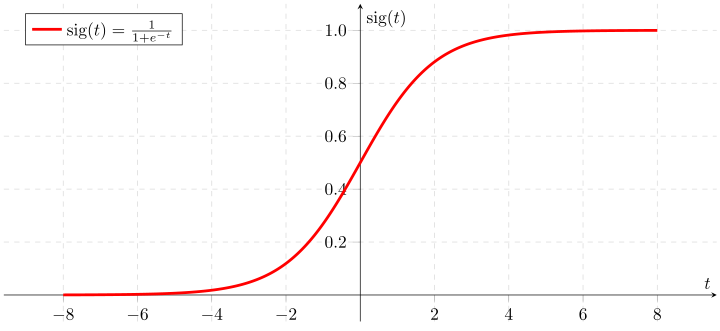
\includegraphics[width=0.7\linewidth]{pics/Sigmoid}
\caption{Graph der Sigmoid-Funktion}
\label{fig:Sigmoid}
\end{figure}
